\documentclass{article}
\usepackage[utf8]{inputenc}

\title{Chem132A Discussion 2 Homework}
\author{Moises Romero (moiseser@uci.edu), Shane Flynn (swflynn@uci.edu) }
\date{10/9/17}


\usepackage{graphicx}
\usepackage{amsmath}
\usepackage{braket}
\usepackage[margin=0.7in]{geometry}


\newcommand{\be}{\begin{equation}}
\newcommand{\ee}{\end{equation}}
\newcommand{\pd}{\partial}

\begin{document}

\maketitle

\section{Path-Dependent and State Functions}
\begin{figure}[h]
\caption{Point 1: (P$_1$,V$_1$,T$_1$), Point 2: (P$_1$,V$_2$,T$_3$), Point 3: (P$_2$,V$_2$,T$_1$), Point 4: (P$_3$,V$_2$,T$_2$)}
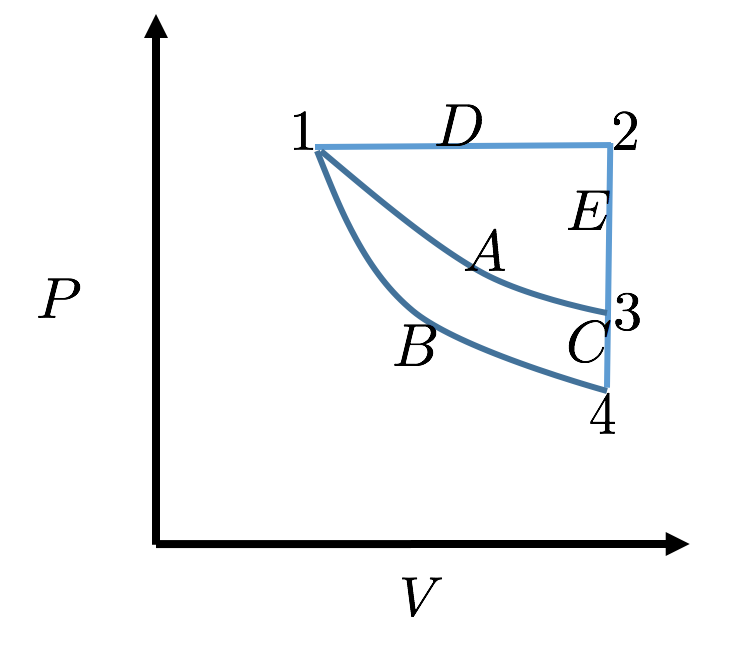
\includegraphics[width=0.5\textwidth]{cycle.png}
\end{figure}
Consider the different pathways as described above in the diagram. 
We are going to calculate the internal energy, heat, and work associated with traveling from point 1 to point 3 (path A). 
Assume an ideal gas for all of the calculations, and that each pathway is done reversibly. 
Physically explain what is happening to the gas along each pathway in the figure after each set of calculations. 

\textbf{Hint:} The Internal Energy of an ideal gas is only a function of Temperature! 
You will need to use this hint to solve this problem, take it as a fact of life (do not worry about proving it). 

\subsection{Pathway 1 $\Rightarrow$ 3}
Starting at Point 1, compute the heat, work, and internal energy associated with traveling pathway A to arrive at point 3.

\subsection{Pathway 1 $\Rightarrow$ 2 $\Rightarrow$ 3}
Starting at Point 1, compute the heat, work, and internal energy associated with traveling pathway D and E to arrive at point 3.
 
 \subsection{Pathway 1 $\Rightarrow$ 4 $\Rightarrow$ 3}
Starting at Point 1, compute the heat, work, and internal energy associated with traveling pathway B and C to arrive at point 3.
Take pathway B to be a reversible, adiabatic expansion. 

 
 
\section{Equations of State and Derivatives}
As discussed in lecture (3 and 4), we can define various derivatives in thermodynamics to describe a physical system. 
These derivatives are chosen to represent interesting quantities, and can sometimes be studied and tabulated. 
In this question we will explore some derivations and applications of these definitions.

\subsection{A Unique EOS}
While we have introduced a few EOS in the course, I am free to define any equation relating state functions (the trick is having a useful definition). 
Consider the arbitrary EOS
\be
\frac{Pv}{RT} = 1 + xP + yP^2
\ee
In this equation x and y are simply constants associated with the chemical system being investigated. 

Use this EOS, compute the isothermal compressibility ($\kappa_T$). 
\be
\kappa_T \equiv -\frac{1}{V}\left(\frac{\pd V}{\pd P}\right)_T
\ee

\subsection{A Familiar EOS}
Using the van der Walls EOS for a gas, compute the isothermal compressibility. 
recall the vdw EOS is given by 
\be
P = \frac{nRT}{(V-nB)} - a\left(\frac{n}{V}\right)^2
\ee

\textbf{HINT:} For any derivative in thermodynamics it turns out that certain relationships are true. 
One of these relationships may be useful for this problem (try using it before anything else).  
\be
\left(\frac{\pd y}{\pd x}\right)_z = \frac{1}{\left(\frac{\pd x}{\pd y}\right)_z}
\ee

\subsection{Internal Pressure}
In Class we defined the Internal Pressure ($\pi_T$) as the following derivative. 
\be
\pi_T \equiv \left(\frac{\pd U}{\pd V}\right)_V
\ee
Through the magic of Calculus it can be shown that
\be
\left(\frac{\pd U}{\pd V}\right)_V = T\left(\frac{\pd P}{\pd T}\right)_V - P
\ee
Using the right hand side of this equation above, compute the Internal Pressure of a van der Walls gas.

\subsection{Application of the Math}
Calculate $\Delta$U$_m$ (the molar internal energy) for the isothermal expansion of nitrogen gas from an initial volume of 1.00 dm$^3$ to 24.8dm$^3$ at 298K. 

\textbf{Hint:} Consider U$\Rightarrow$U(T,V) and write the total differential. 

\section{Fitting Parameters}
In question 2 we derived analytic expressions for the isothermal compressibility ($\kappa_T$) for two different equations of state.
(Before trying this problem, you may want to speak with a TA to see if your equations are correct). 

\subsubsection*{Argon}
Consider Argon, whose van der Walls parameters are
\be
a = 1.355 \frac{\text{Bar-}L^2}{\text{mol}^2} \qquad b = 0.03201 \frac{L}{\text{mol}}
\ee
Compute the isothermal compressibility for argon over a range of temperatures (250K to 350K at increments of 10 for example). 
To make life simple set the volume, and moles to 1. 
Make a plot of of $\kappa_T$ vs T for your calculations. 

\subsection{Arbitrary EOS}
Now that we have values for the compressibility see if you can determine a parameter y that is consistent with your previous results determined by the van der Walls EOS. 
Set the pressure, and volume to 1 for convenience. 
Make a plot of the arbitrary parameter y vs T and see what it looks like.

\end{document}